\documentclass{article}
\usepackage{graphicx} % Required for inserting images

\title{Formato para librerias GIOC}
\author{Amado A. Cabrera}
\date{July 2025}

\begin{document}

\maketitle

\begin{enumerate}
\item Usar de las funciones de ForScience para formatear bonito los mensajes
de uso 
\item Nombres de funciones claros y explícitos según lo que hagan
\item Mensajes de uso en la forma estándar de Mathematica, siendo claros con 
los argumentos de las funciones y qué retorna
\item Breaks obligatorios antes de las 80 columnas
\item Si la función tiene opciones. Colocar al final de la definición de la primer
definición de uso (capaz tiene más de una definición las opciones disponibles
\end{enumerate}

\begin{figure}
\centering
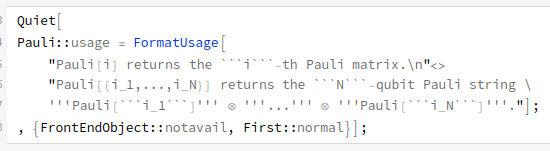
\includegraphics[width=\textwidth]{estandar1.png}
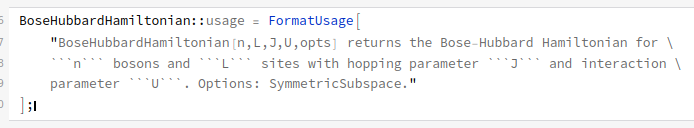
\includegraphics[width=\textwidth]{estandar2.png}
\end{figure}

\end{document}
